\documentclass[12pt, a4paper, twoside]{scrartcl}
 %---- Allgemeine Layout Einstellungen ------------------------------------------

% Für Kopf und Fußzeilen, siehe auch KOMA-Skript Doku
\usepackage[komastyle]{scrpage2}
\pagestyle{scrheadings}
\setheadsepline{0.5pt}[\color{black}]


%Einstellungen für Figuren- und Tabellenbeschriftungen
\setkomafont{captionlabel}{\sffamily\bfseries}
\setcapindent{0em}


%---- Weitere Pakete -----------------------------------------------------------
% Die Pakete sind alle in der TeX Live Distribution enthalten. Wichtige Adressen
% www.ctan.org, www.dante.de

% Sprachunterstützung
\usepackage[ngerman]{babel}

% Benutzung von Umlauten direkt im Text
% entweder "latin1" oder "utf8"
\usepackage[utf8]{inputenc}

% Pakete mit Mathesymbolen und zur Beseitigung von Schwächen der Mathe-Umgebung
\usepackage{latexsym,exscale,stmaryrd,amssymb,amsmath}

% Weitere Symbole
\usepackage[nointegrals]{wasysym}
\usepackage{eurosym}

% Anderes Literaturverzeichnisformat
%\usepackage[square,sort&compress]{natbib}

% Für Farbe
\usepackage{color}

% Zur Graphikausgabe
%Beipiel: \includegraphics[width=\textwidth]{grafik.png}
\usepackage{graphicx}

% Text umfließt Graphiken und Tabellen
% Beispiel:
% \begin{wrapfigure}[Zeilenanzahl]{"l" oder "r"}{breite}
%   \centering
%   \includegraphics[width=...]{grafik}
%   \caption{Beschriftung} 
%   \label{fig:grafik}
% \end{wrapfigure}
\usepackage{wrapfig}

% Mehrere Abbildungen nebeneinander
% Beispiel:
% \begin{figure}[htb]
%   \centering
%   \subfigure[Beschriftung 1\label{fig:label1}]
%   {\includegraphics[width=0.49\textwidth]{grafik1}}
%   \hfill
%   \subfigure[Beschriftung 2\label{fig:label2}]
%   {\includegraphics[width=0.49\textwidth]{grafik2}}
%   \caption{Beschriftung allgemein}
%   \label{fig:label-gesamt}
% \end{figure}
\usepackage{subfigure}

% Caption neben Abbildung
% Beispiel:
% \sidecaptionvpos{figure}{"c" oder "t" oder "b"}
% \begin{SCfigure}[rel. Breite (normalerweise = 1)][hbt]
%   \centering
%   \includegraphics[width=0.5\textwidth]{grafik.png}
%   \caption{Beschreibung}
%   \label{fig:}
% \end{SCfigure}
\usepackage{sidecap}
\usepackage{float}

% Befehl für "Entspricht"-Zeichen
\newcommand{\corresponds}{\ensuremath{\mathrel{\widehat{=}}}}
\newcommand{\folgt}{\ensuremath{\mathrel{\Rightarrow}}}
\newcommand{\equals}{\ensuremath{\mathrel{\Leftrightarrow}}}
\newcommand{\degree}{\ensuremath{\mathrel{^{\circ}}}}

\newcommand{\nn}{\nonumber}
\newcommand{\tn}[1]{\textnormal{#1}}
\newcommand{\D}{\ensuremath{\mathrel{\rm d}}}

\newcommand{\const}{\tn{const}}

\newcommand{\meter}{\ensuremath{\mathrel{\tn m}}}
\newcommand{\kilogramm}{\ensuremath{\mathrel{\tn{kg}}}}
\newcommand{\second}{\ensuremath{\mathrel{\tn s}}}
\newcommand{\sekunde}{\second}

\newcommand{\volt}{\ensuremath{\mathrel{\tn V}}}
\newcommand{\pascal}{\ensuremath{\mathrel{\tn{Pa}}}}
\newcommand{\coulomb}{\ensuremath{\mathrel{\tn C}}}
\newcommand{\newton}{\ensuremath{\mathrel{\tn N}}}
\newcommand{\liter}{\ensuremath{\mathrel{\tn l}}}
\newcommand{\celsius}{\ensuremath{\mathrel{\tn C}}}
\newcommand{\fahrenheit}{\ensuremath{\mathrel{\tn F}}}
\newcommand{\joule}{\ensuremath{\mathrel{\tn J}}}
\newcommand{\kelvin}{\ensuremath{\mathrel{\tn K}}}
\newcommand{\mol}{\ensuremath{\mathrel{\tn{mol}}}}
\newcommand{\gramm}{\ensuremath{\mathrel{\tn{g}}}}

\newcommand{\kilo}{\ensuremath{\mathrel{\tn k}}}
\newcommand{\hecto}{\ensuremath{\mathrel{\tn h}}}

\newcommand{\centi}{\ensuremath{\mathrel{ \tn c}}}
\newcommand{\milli}{\ensuremath{\mathrel{ \tn m}}}
\newcommand{\micro}{\ensuremath{\mathrel{ \tn\mu }}}



%\newcommand{}{\ensuremath{\mathrel{  }}}
%\newcommand{}{\ensuremath{\mathrel{  }}}
%\newcommand{}{\ensuremath{\mathrel{  }}}


\newcommand{\person}[1]{\textsc{#1}}

 \begin{document}
 %Titelseite
\begin{titlepage}
\centering
\textsc{\Large Anfängerpraktikum der Fakultät für
  Physik,\\[1.5ex] Universität Göttingen}

\vspace*{4.2cm}

\rule{\textwidth}{1pt}\\[0.5cm]
{\huge \bfseries
  Spezifische Wärme der Luft und Gasthermometer}\\[0.5cm]
\rule{\textwidth}{1pt}

\vspace*{3.5cm}

\begin{Large}
\begin{tabular}{ll}
Praktikanten: &  Silke Andrea Teepe\\
& Marcel Kramer\\
E-Mail: & \\
Betreuer: & Alexander Schmelev\\
\end{tabular}
\end{Large}

\vspace*{0.8cm}

\begin{Large}
\fbox{
  \begin{minipage}[t][2.5cm][t]{6cm} 
    Testat:
  \end{minipage}
}
\end{Large}

\end{titlepage}
\cleardoublepage
\tableofcontents
\cleardoublepage
\setcounter{page}{1}

\section{Einleitung}
\label{sec:einleitung}


\section{Theorie}
\label{sec:theorie}

\subsection{Gasthermometer}
Das Gasthermometer oder auch \person{Jolly}sche Luftthermometer ist ein Glaskolben der luftdicht an digitales Differenzdruckmessgerät angeschlossen ist. Das Messgerät zeigt nun die Druckdifferenz $\Delta p$ zwischen Umgebungsdruck $p_0$ und dem Druck $p$ im Glaskolben an. Im Kolben herscht folglich ein Druck von
\begin{align}
 p = p_0 + \Delta p \nn
\end{align}
Durch Temperaturänderungen ändert sich der Druck im Kolben und man kann mittels der in Kapitel \ref{subsec:theorie_eigenschaften_ideales_gas} beschrieben Formeln u.A. die Temperaturänderungen berechnen.

\subsection{Innere Energie eines Gases}
Die Moleküle in einem Idealen Gas werden als Punktförmig angesehen und es wird davon ausgegangen, dass es keine Wechselwirkungen innerhalb des Gases gibt.
Folglich ist die gesammte innere Energie $U$ des Gases die Summe der kinetischen Energie $E_{kin}$ der Moleküle. Mit der Temperatur $T$ als Maß der mittleren Energie der Moleküle gilt somit
\begin{align}
 E_{kin} = \frac{1}{2}\cdot m\cdot v^{2} = \frac{3}{2}\cdot k_B\cdot T \nn
\end{align}
mit der Bolzmannkonstante $k_B=1.381\cdot 10^{-23} \frac{\joule}{\kelvin}$
\\
Für einen realen Stoff gibt es neben den 3 Freiheitsgraden für Translation noch bis zu 3 Freiheitsgrade für Rotation bzw. 3 für Schwingungen.
Auf jeden dieser Freiheitsgrade entfällt somit die Energie
\begin{align}
 E = \frac{1}{2}\cdot k_B\cdot T \nn
\end{align}
Folglich hat ein Gas mit $N$ Molekülen und $f$ Freiheitsgraden die innere Energie
\begin{align}
 U = \frac{f}{2}\cdot N\cdot k_B\cdot T = \frac{f}{2}\cdot n\cdot R\cdot T \label{eq:U}
\end{align}
mit $n = \frac{N}{N_A}$ der Stoffmenge in $\mol$ und  der Gaskonstanten $R = N_A\cdot k_B$

\subsection{Eigenschaften eines Idealen Gases}
\label{subsec:theorie_eigenschaften_ideales_gas}
Der Zustand eines Idealen Gases kann durch die Größen Druck $p$, Volumen $V$ und Temperatur $T$ vollständig beschrieben werden.
Für eine Stoffmenge $n$ eines Idealen Gases gilt die Zustandsgleichung
\begin{align}
 p\cdot V = n\cdot R\cdot T \label{eq:zustandsgleichung}
\end{align}
Folglich gilt
\begin{align*}
 p &\propto T \tn{\;\; bei konstantem Volumen } V, \\
 V &\propto T \tn{\;\; bei konstantem Druck } p 
\end{align*}
und nach den Gesetzen von \person{Gay-Lussac} und \person{Boyle-Mariotte} gilt
\begin{align*}
 p\left(\vartheta\right) &= p_0\cdot\left[1+\beta\vartheta\right] \\
 V\left(\vartheta\right) &= V_0\cdot\left[1+\beta\vartheta\right]
\end{align*}
mit der Temperatur $\vartheta$ in $\degree\celsius$ und $\beta = \frac{1}{273.15 \degree\celsius}$ \footnote{Nach P. Schaaf (2014): ”Das Physikalische Praktikum”, Universitätsverlag Göttingen}.
Folglich hat ein Ideales Gas beim absoluten Nullpunkt von $-\frac{1}{\beta} = -273.15 \degree\celsius$ weder ein Volumen noch übt es einen Druck aus.

\subsection{Spezifische Wärme}
\subsubsection*{Isochore Temperaturänderung}
Der erste Hauptsatz der Wärmelehre besagt für die Änderung der inneren Energie $\Delta U$ eines abgeschlossenen Systems
\begin{align}
 \Delta U &= \Delta Q + \Delta W \label{eq:HS} \\
\equals \Delta Q &= \Delta U - \Delta W \nn 
\end{align}
mit $\Delta Q$ der hinzugefügten Wärmeenergie und $\Delta W = -p \Delta V$ der aufgebrachten Arbeit.
Bei einer isochoren Erwärmung, also bei $V = \const$ und damit $\Delta W = -p \Delta V = 0$, ist $\Delta U = \Delta Q$.
Aus Gleichung \eqref{eq:U} folgt für eine Temperaturänderung $\Delta T$ somit
\begin{align}
 \Delta Q = \Delta U = \frac{f}{2}\cdot n \cdot R \cdot \Delta T
\end{align}
Das Verhältnis
\begin{align}
 c_V &= \frac{\Delta Q}{\Delta T \cdot n} = \frac{f}{2} \cdot R \nn
%  \folgt \frac{c_V}{R} &= \frac{f}{2} \nn
\end{align}
bezeichnet die spezifische Wärmekapazität von einem Mol eines Gases (in $\frac{\joule}{\kelvin\cdot\mol}$).
Damit ergibt sich die Gleichung für die benötigte Energie einer isochoren Erwärmung um $\Delta T$
\begin{align}
 \Delta U = \left(\Delta Q\right)_V = n\cdot c_V \cdot \Delta T \label{eq:dU_V}
\end{align}

\subsubsection*{Isobare Temperaturänderung}
Wenn der Druck konstant beleibt aber nicht das Volumen, also eine isobare Erwärmung, muss zusätzlich noch die Volumenarbeit $p \cdot\Delta V$ aufgebracht werden.
Nach der Gleichung \eqref{eq:zustandsgleichung} ergibt sich
\begin{align}
 p\cdot\Delta V = n\cdot R\cdot \Delta T
\end{align}
Aus dem Hauptsatz folgt somit
\begin{align}
 \Delta Q &= \Delta U - \Delta W \nn\\
          &= \frac{f}{2} \cdot n\cdot R\cdot \Delta T + n\cdot R\cdot \Delta T \nn\\
          &= \left(\frac{f}{2}+1\right) \cdot n\cdot R\cdot \Delta T \nn\\
          &= c_p \cdot n\cdot \Delta T
\end{align}

Damit ergibt sich die Beziehung zwischen $c_p$ und $c_V$:
\begin{align}
 c_p = \left(\frac{f}{2}+1\right) \cdot R = c_V + R \nn
\end{align}

\subsubsection*{Gleichung für Freiheitsgrade}
Wenn keine Zustandgröße konstant beleibt gilt nach der Zustandsgleichung
\begin{align}
 \D \left(p\cdot V\right) &= n\cdot R\cdot \D T \nn\\
 \folgt \frac{\D p \cdot V + p \cdot \D V}{R} &= n \cdot \D T \label{eq:n_dT}
\end{align}
Aus den Gleichungen \eqref{eq:n_dT}, \eqref{eq:dU_V} und dem Hauptsatz folgt
\begin{align}
 \Delta Q &= \Delta U - \Delta W \nn\\
          &= c_V\cdot n\cdot \Delta T + p \cdot \Delta V \nn\\
          &= c_V \cdot \frac{\Delta p \cdot V + p \cdot \Delta V}{R} + p\cdot \Delta V \nn\\
 \folgt
 \Delta Q - p \cdot \Delta V &= \left(\Delta p \cdot V + p \cdot \Delta V\right)\cdot \frac{c_V}{R} \nn\\
 \folgt
 \frac{\Delta Q - p \cdot \Delta V}{\Delta p \cdot V + p \cdot \Delta V} &= \frac{c_V}{R} = \frac{f}{2}
\end{align}

\subsection{Kondensator}
Beim Aufladen eines Kondensator mit der Kapazität $C$ muss die Ladung $\Delta q$ die bereits aufgebaute Spannung $U = \frac{q}{C}$ überwinden. Dazu wird die Energie $\Delta E = \Delta q\cdot \frac{q}{C}$ benötigt.
Somit ist die Gesamtenergie $E$ im Kondensator der von $Q_0 = 0$ bis $Q_{max} = U \cdot C$ aufgeladen wird
\begin{align}
 E &= \int_{0}^{Q_{max}} \frac{q}{C}\cdot \D q \nn\\
   &= \frac{1}{2}\cdot\frac{Q_{max}^2}{C} \nn\\
   &= \frac{1}{2}\cdot C\cdot U^2
\end{align}



\section{Durchführung}
\label{sec:durchfuehrung}
\subsection{Gasthermometer}
\begin{figure}[h!]
	\centering
	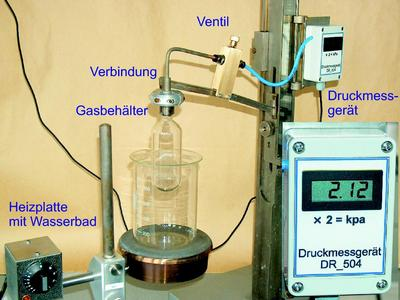
\includegraphics[scale=1]{Gasthermometer.png}
	\caption{Versuchsaufbau Gasthermometer\protect\footnotemark} 
\end{figure}
\footnotetext{https://lp.uni-goettingen.de/get/text/3643 Abb.3723}
Da das Druckmessgerät nicht in der Lage ist, negative  Druckdifferenzen zu erfassen, wird zunächst das Ventil geöffnet und im Glaskolben Luftdruck hergestellt. Mit Hilfe von Eiswasser wird dann der Kolben auf etwa $0\degree\celsius$ abgekühlt und anschließend das Ventil wieder verschlossen. Das Druckmessgerät sollte nun ca. $0.00\kilo\pascal$ anzeigen. \\
Nun bestimmt man den Druck $p_V \left( T \right)$ der Luft im Kolben für konstantes Volumen $V$ und Temperaturen zwischen $0\degree\celsius$ und $100\degree\celsius$, sowohl für Erwärmen, als auch Abkühlen des Kolbens. Dabei sollten Schritte von $\Delta T \le 5K $ gewählt werden. Um eine möglichste gleichförmige Temperaturänderung zu gewährleisten sollte das Wasserbad dauernd umgerührt werden.

\subsection{Spezifische Wärme der Luft}
\begin{figure}[h!]
	\centering
	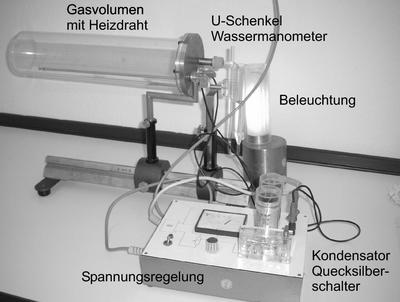
\includegraphics[scale=1]{SpezWaerme.png}
	\caption{Versuchsaufbau Spez. Wärme d. Luft \protect\footnotemark}
\end{figure}
\footnotetext{https://lp.uni-goettingen.de/get/text/3643 Abb.3724}
Ein Zylinder gefüllt mit Luft ist mit einem Wassermanometer verbunden. An dass Gasvolumen kann über einen Kondensator und einen Glühdraht eine spezifische Wärmemenge $Q$ abgegeben werden. Das Gasvolumen kann bei Vernachlässigung der Manometeränderung als konstant angesehen werden und somit die Druckänderung am Manometer abgelesen werden. \\
Der Kondensator wird aufgeladen und dann über den Heizdraht entladen. Dabei wird der maximale Ausschlag $\Delta p$ des Manometers abgelesen. Dieser wird für mehrfach für möglichst viele Spannungen zwischen 100V und 500V gemessen. Außerdem ist das Innenvolumen $V$ des Zylinders zu messen. \\
Während der Messung ist mit dem Ventil die Belüftungsöffnung des Zylinders zu verschließen und zwischen den Messungen beim Temperaturausgleich zu öffnen. Nach Beendigung der Messungen ist das Ventil geöffnet zurückzulassen.

\section{Auswertung}
\label{sec:auswertung}


\section{Diskussion}
\label{sec:diskussion}

\end{document}
